\subsection{PB}
Il preventivo di questa macrofase è stato stilato durante la precedente fase "baseline delle tecnologie" (della macrofase RTB) considerando anche i risparmi iniziali e rivalutando la ripartizione iniziale delle ore nei vari ruoli (scritte nel documento \emph{Candidatura.pdf}), per i dettagli sulla nuova ripartizione delle ore si legga la sezione \$6.1.4.4.
\subsubsection{Requisiti Obbligatori}
\paragraph{Incremento 1}
\subparagraph{Prospetto Orario}
\begin{center}
	\renewcommand{\arraystretch}{1.8} %aumento ampiezza righe
	\begin{tabular}{ |m{10em}|c|c|c|c|c|c|c| }
	\hline
	\textbf{Membro} & \textbf{Re} & \textbf{Am} &  \textbf{An} &  \textbf{Pt} &  \textbf{Pg} &  \textbf{Ve} &  \textbf{Totale}\\
    \hline
    Irene Benetazzo   & - & - & - & 8 & 5 & 3 & \textbf{16} \\
    \hline
    Tommaso Berlaffa  & 3 & - & - & - & 10 & - & \textbf{13} \\
    \hline
    Mattia Episcopo   & - & 4 & - & 7 & 4 & 2 & \textbf{17} \\
    \hline
    Pietro Macrì      & - & 4 & - & 5 & 7 & 2 & \textbf{18} \\
    \hline
    Qi Fan Andrea Pan & - & - & - & 7 & 7 & 3 & \textbf{17} \\
    \hline
    Matteo Pillon     & - & - & - & 5 & 8 & 3 & \textbf{16} \\
    \hline
    Samuele Rizzato   & - & - & - & 8 & 5 & 3 & \textbf{16} \\
    \hline
    \textbf{Totale ore} & \textbf{3} & \textbf{8} &  \textbf{0} &  \textbf{40} &  \textbf{46} &  \textbf{16} &  \textbf{113}\\
    \hline
	\end{tabular}
\end{center}
\begin{figure}[H]
   \centering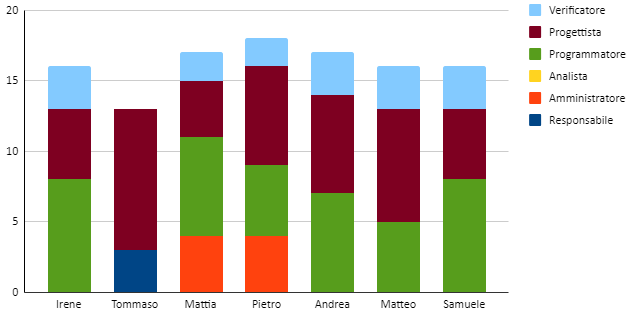
\includegraphics{images/preventivo/PB-incremento1-ore.png}
   \caption{PB-Incremento 1 - preventivo ripartizione oraria}
\end{figure}


\subparagraph{Prospetto Economico}
\begin{center}
	\renewcommand{\arraystretch}{1.8} %aumento ampiezza righe
	\begin{tabular}{ |m{10em}|c|c|c|c|c|c|c| }
	\hline
	\textbf{Ruolo} & \textbf{Re} & \textbf{Am} &  \textbf{An} &  \textbf{Pt} &  \textbf{Pg} &  \textbf{Ve} &  \textbf{Totale}\\
    \hline
    Totale ore & 3 & 8 & 0 & 40 & 46 & 16 & \textbf{113}\\
    \hline
    Costo \euro/h & 30\euro/h & 20\euro/h & 25\euro/h & 25\euro/h & 15\euro/h & 15\euro/h & \\
    \hline
    \textbf{Totale costo} & \textbf{90\euro} & \textbf{160\euro} &  \textbf{0\euro} &  \textbf{1000\euro} &  \textbf{690\euro} &  \textbf{240\euro} &  \textbf{2180\euro}\\
    \hline
	\end{tabular}

    \begin{figure}[H]
       \centering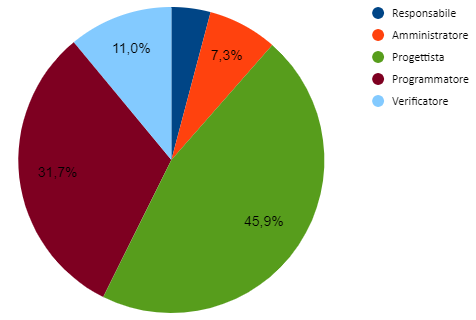
\includegraphics{images/preventivo/PB-incremento1-costo.png}
       \caption{PB-Incremento 1 - preventivo ripartizione economica}
    \end{figure}
\end{center}



\paragraph{Incremento 2}
\subparagraph{Prospetto Orario}
\begin{center}
	\renewcommand{\arraystretch}{1.8} %aumento ampiezza righe
	\begin{tabular}{ |m{10em}|c|c|c|c|c|c|c| }
	\hline
	\textbf{Membro} & \textbf{Re} & \textbf{Am} &  \textbf{An} &  \textbf{Pt} &  \textbf{Pg} &  \textbf{Ve} &  \textbf{Totale}\\
    \hline
    Irene Benetazzo   & - & - & - & 7 & 5 & 3 & \textbf{15} \\
    \hline
    Tommaso Berlaffa  & - & - & - & 6 & 6 & 3 & \textbf{15} \\
    \hline
    Mattia Episcopo   & 3 & - & - & - & 10 & - & \textbf{13} \\
    \hline
    Pietro Macrì      & - & - & - & 5 & 6 & 3 & \textbf{14} \\
    \hline
    Qi Fan Andrea Pan & - & 4 & - & 4 & 8 & 2 & \textbf{18} \\
    \hline
    Matteo Pillon     & - & - & - & 6 & 7 & 3 & \textbf{16} \\
    \hline
    Samuele Rizzato   & - & 5 & - & 6 & 5 & 3 & \textbf{19} \\
    \hline
    \textbf{Totale ore} & \textbf{3} & \textbf{9} &  \textbf{0} &  \textbf{34} &  \textbf{47} &  \textbf{17} &  \textbf{110}\\
    \hline
	\end{tabular}
\end{center}
\begin{figure}[H]
   \centering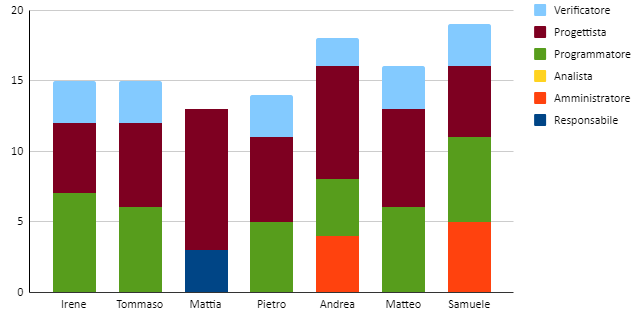
\includegraphics{images/preventivo/PB-incremento2-ore.png}
   \caption{PB-Incremento 2 - preventivo ripartizione oraria}
\end{figure}

\subparagraph{Prospetto Economico}
\begin{center}
	\renewcommand{\arraystretch}{1.8} %aumento ampiezza righe
	\begin{tabular}{ |m{10em}|c|c|c|c|c|c|c| }
	\hline
	\textbf{Ruolo} & \textbf{Re} & \textbf{Am} &  \textbf{An} &  \textbf{Pt} &  \textbf{Pg} &  \textbf{Ve} &  \textbf{Totale}\\
    \hline
    Totale ore & 3 & 9 & 0 & 34 & 47 & 17 & \textbf{110}\\
    \hline
    Costo \euro/h & 30\euro/h & 20\euro/h & 25\euro/h & 25\euro/h & 15\euro/h & 15\euro/h & \\
    \hline
    \textbf{Totale costo} & \textbf{90\euro} & \textbf{180\euro} &  \textbf{0\euro} &  \textbf{1190\euro} &  \textbf{705\euro} &  \textbf{255\euro} &  \textbf{2420\euro}\\
    \hline
	\end{tabular}

    \begin{figure}[H]
       \centering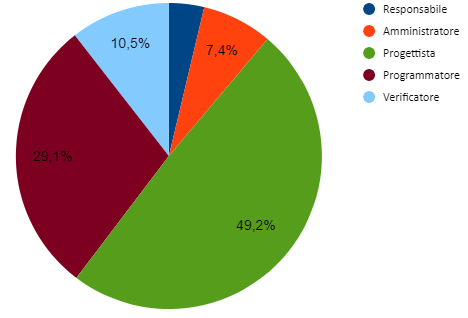
\includegraphics{images/preventivo/PB-incremento2-costo.png}
       \caption{PB-Incremento 2 - preventivo ripartizione economica}
    \end{figure}
\end{center}


\subsubsection{Requisiti Desiderabili}
\paragraph{Incremento 3}
\subparagraph{Prospetto Orario}
\begin{center}
	\renewcommand{\arraystretch}{1.8} %aumento ampiezza righe
	\begin{tabular}{ |m{10em}|c|c|c|c|c|c|c| }
	\hline
	\textbf{Membro} & \textbf{Re} & \textbf{Am} &  \textbf{An} &  \textbf{Pt} &  \textbf{Pg} &  \textbf{Ve} &  \textbf{Totale}\\
    \hline
    Irene Benetazzo   & - & - & - & 4 & 5 & 3 & \textbf{12} \\
    \hline
    Tommaso Berlaffa  & - & - & - & 5 & 4 & 3 & \textbf{12} \\
    \hline
    Mattia Episcopo   & - & 5 & - & 3 & 5 & 2 & \textbf{15} \\
    \hline
    Pietro Macrì      & 3 & - & - & - & 7 & - & \textbf{10} \\
    \hline
    Qi Fan Andrea Pan & - & - & - & 4 & 5 & 3 & \textbf{12} \\
    \hline
    Matteo Pillon     & - & 4 & - & 5 & 3 & 2 & \textbf{14} \\
    \hline
    Samuele Rizzato   & - & - & - & 5 & 5 & 3 & \textbf{13} \\
    \hline
    \textbf{Totale ore} & \textbf{3} & \textbf{9} &  \textbf{0} &  \textbf{26} &  \textbf{34} &  \textbf{16} &  \textbf{88}\\
    \hline
	\end{tabular}
\end{center}
\begin{figure}[H]
   \centering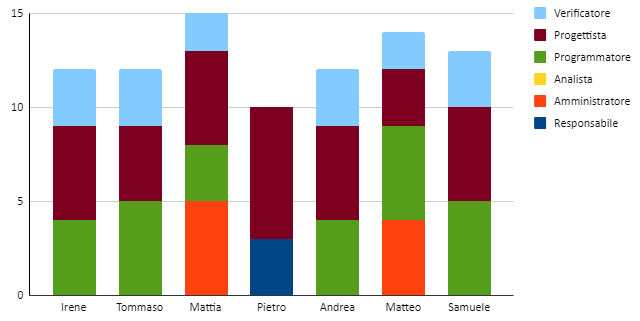
\includegraphics{images/preventivo/PB-incremento3-ore.png}
   \caption{PB-Incremento 3 - preventivo ripartizione oraria}
\end{figure}


\subparagraph{Prospetto Economico}
\begin{center}
	\renewcommand{\arraystretch}{1.8} %aumento ampiezza righe
	\begin{tabular}{ |m{10em}|c|c|c|c|c|c|c| }
	\hline
    Totale ore & 3 & 9 & 0 & 26 & 34 & 16 & \textbf{88}\\
    \hline
    Costo \euro/h & 30\euro/h & 20\euro/h & 25\euro/h & 25\euro/h & 15\euro/h & 15\euro/h & \\
    \hline
    \textbf{Totale costo} & \textbf{90\euro} & \textbf{180\euro} &  \textbf{0\euro} &  \textbf{650\euro} &  \textbf{510\euro} &  \textbf{240\euro} &  \textbf{1730\euro}\\
    \hline
	\end{tabular}

    \begin{figure}[H]
       \centering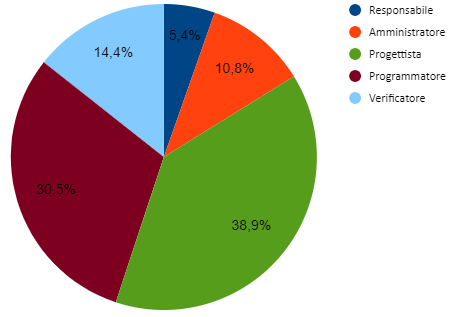
\includegraphics{images/preventivo/PB-incremento3-costo.png}
       \caption{PB-Incremento 3 - preventivo ripartizione economica}
    \end{figure}
\end{center}



\paragraph{Incremento 4}
\subparagraph{Prospetto Orario}
\begin{center}
	\renewcommand{\arraystretch}{1.8} %aumento ampiezza righe
	\begin{tabular}{ |m{10em}|c|c|c|c|c|c|c| }
	\hline
	\textbf{Membro} & \textbf{Re} & \textbf{Am} &  \textbf{An} &  \textbf{Pt} &  \textbf{Pg} &  \textbf{Ve} &  \textbf{Totale}\\
    \hline
    Irene Benetazzo   & - & 5 & - & 4 & 4 & 2 & \textbf{15} \\
    \hline
    Tommaso Berlaffa  & 1 & 4 & - & 4 & 4 & 3 & \textbf{16} \\
    \hline
    Mattia Episcopo   & 1 & - & - & 5 & 4 & 3 & \textbf{13} \\
    \hline
    Pietro Macrì      & 1 & - & - & 6 & 5 & 3 & \textbf{15} \\
    \hline
    Qi Fan Andrea Pan & 1 & - & - & 4 & 5 & 3 & \textbf{13} \\
    \hline
    Matteo Pillon     & 3 & 2 & - & - & 7 & - & \textbf{12} \\
    \hline
    Samuele Rizzato   & 1 & - & - & 4 & 5 & 3 & \textbf{13} \\
    \hline
    \textbf{Totale ore} & \textbf{8} & \textbf{11} &  \textbf{0} &  \textbf{27} &  \textbf{34} &  \textbf{17} &  \textbf{97}\\
    \hline
	\end{tabular}
\end{center}
\begin{figure}[H]
   \centering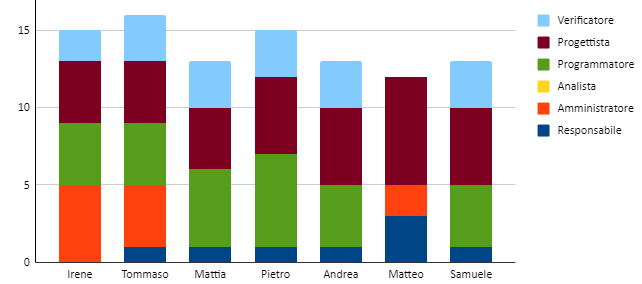
\includegraphics{images/preventivo/PB-incremento4-ore.png}
   \caption{PB-Incremento 4 - preventivo ripartizione oraria}
\end{figure}


\subparagraph{Prospetto Economico}
\begin{center}
	\renewcommand{\arraystretch}{1.8} %aumento ampiezza righe
	\begin{tabular}{ |m{10em}|c|c|c|c|c|c|c| }
	\hline
	\textbf{Ruolo} & \textbf{Re} & \textbf{Am} &  \textbf{An} &  \textbf{Pt} &  \textbf{Pg} &  \textbf{Ve} &  \textbf{Totale}\\
    \hline
    Totale ore & 8 & 11 & 0 & 27 & 34 & 17 & \textbf{97}\\
    \hline
    Costo \euro/h & 30\euro/h & 20\euro/h & 25\euro/h & 25\euro/h & 15\euro/h & 15\euro/h & \\
    \hline
    \textbf{Totale costo} & \textbf{240\euro} & \textbf{220\euro} &  \textbf{0\euro} &  \textbf{675\euro} &  \textbf{510\euro} &  \textbf{255\euro} &  \textbf{1900\euro}\\
    \hline
	\end{tabular}

    \begin{figure}[H]
       \centering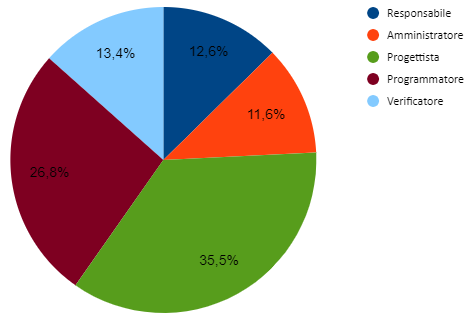
\includegraphics{images/preventivo/PB-incremento4-costo.png}
       \caption{PB-Incremento 4 - preventivo ripartizione economica}
    \end{figure}
\end{center}

\newpage